\subsection{Niveles.} \label{Niveles}
Yolotl es un juego compuesto por diez niveles: un nivel introductorio y los nueve 
niveles del inframundo.  Dado que la idea concepto del juego Yolotl lo situa en 
el Mictlán, la cantidad mínima esperados seria nueve; sin embargo, se tomó la 
decisión de incluir un nivel de introducción debido a los siguientes factores: 

\begin{itemize}
	\item Introducir al jugador a las mecánicas de juego básicas antes de lanzarlo 
	a un nivel más complicado.
	\item Situar el juego dentro de un contexto histórico real, permitiéndole al 
	jugador conocer sobre la sociedad Mexica de una manera en la que el jugador 
	pueda ser participe de este contexto histórico.
	\item Seguir una estructura narrativa básica en la que se presente la vida 
	cotidiana del héroe antes del llamado a la aventura \cite{RefHeroe}.
\end{itemize}

Usualmente, en el juego de Yolotl, un nivel está compuesto de dos secciones: una 
sección de obstáculos y plataformas en donde cumplirá un objetivo propio del nivel 
y otra donde el jugador se enfrentará al enemigo jefe del nivel. A excepción 
del primero y ultimo nivel el resto de los niveles siguen esa estructura. En el 
caso del primer nivel sigue la división de las dos secciones, con la diferencia 
de que no existe un enemigo jefe a vencer en la segunda sección del nivel; 
mientras que en el último nivel existe una única sección en donde el jugador 
se enfrentará a las diferentes transformaciones del jefe final.
\\
\par
La progresión entre niveles es lineal (Ver figura \ref{fig:ProgreNiveles}), 
por lo que no se puede acceder al nivel determinado sin antes haber completado 
a su predecesor; siendo el primer nivel, el que se encuentra disponible de manera 
estándar al empezar una nueva partida. Un nivel se da completado únicamente 
hasta que se ha derrotado al enemigo jefe del nivel; salvo por el primer nivel, 
el cual se considera terminado una vez que el jugador obtiene el arma de la 
protagonista. Cuando el jugador completa un nivel, además de desbloquear el 
siguiente nivel, el jugador podrá ver determinadas cinemáticas con las que podrá 
seguir la historia del juego y obtiene mejoras sobre alguno de los atributos del 
personaje.
\\
\par
En la tabla se encuentra información referente a cada nivel tal como los 
objetivos a cumplir, el enemigo a vencer, lo que se obtiene al completar el nivel.

%%============== PROGRECION DE NIVELES ==============
\begin{figure}
  \centering
   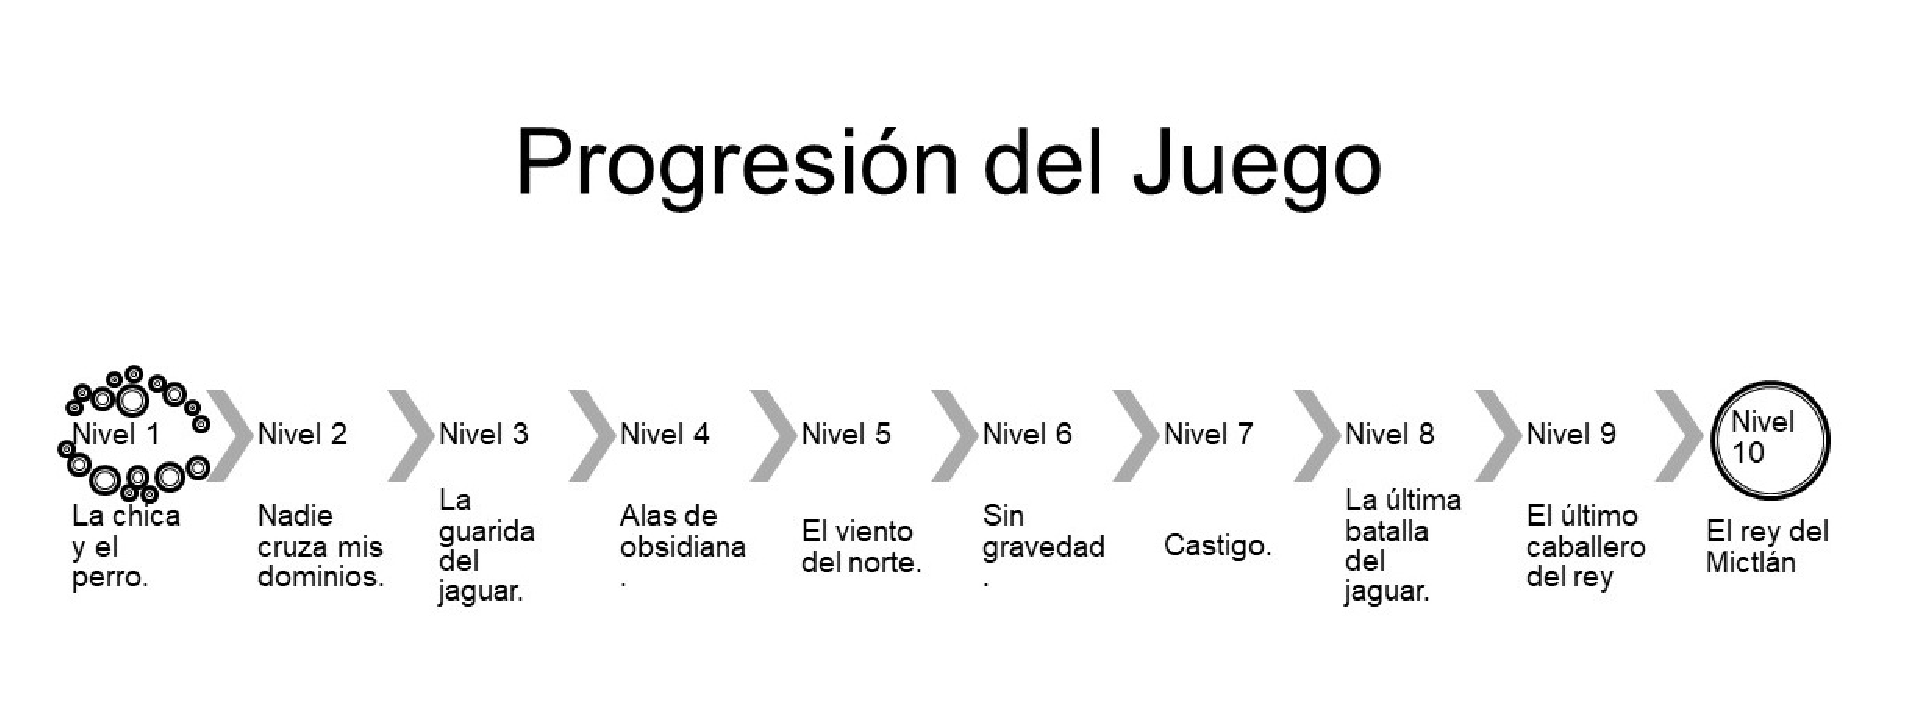
\includegraphics[width=0.8 \textwidth]{05TrabajoRealizado/01DocDiseno02/imagenes/ProgresJuego}
  \caption{Progresión del juego}
  \label{fig:ProgreNiveles}
\end{figure} 

%%============== TABLA DE NIVELES =============
%\begin{table}
	\begin{longtable}[c]{ | m{3.75cm} | m{3.75cm}| m{3.75cm} | m{3.75cm}|} 
		%\endhead		
		%\endfirsthead
		%\endlastfoot
		%\hline
		\rowcolor{cyan} Nivel.& Objetivo & Zona de plataformas	Enemigo jefe & Progreso obtenido. \\ 
		\hline
		%-------------------------------
		Nivel 1 “La chica y el perro”. & 
		Hablar con al menos cuatro ciudadanos.
			\par 
			Interactuar con Xólotl.
			\par 
			Obtener la caracola.&
		Sin enemigo jefe.&
		 Nivel 1.
			\par 
			Cinemática 3.
			\par 
			Cinemática 4.
			\par 
			Habilidad de disparo.		 
		 \\ 
		\hline
		%-------------------------------
		Nivel 2 “Nadie cruza mis dominios”. & 
		Atravesar el rio evitando tocar a los Xoloitzcuintles, por cada Xoloitzcuintles tocado incrementara el poder de Xochitónal. &
		Xochitónal. &
		Mejora en la cantidad de vida de Malinalli.
			\par 
			Cinemática 6.
			\par 
			Cinemática 7.
			\par 
			Cinemática 8.
			\par 
			Cinemática 9.
			\par 
			Cinemática 10.
			\par 
			Nivel 3.		 
		 \\ 
		\hline
		%-------------------------------
		Nivel 3 “La guarida del jaguar”. & 
		Llegar a la guarida de Tepeyóllotl. &
		Tepeyóllotl. &
		Mejora en la cantidad de Tonalli de Malinalli.
			\par 
			Cinemática 12.
			\par
			Cinemática 13.
			\par 
			Cinemática 14.
			\par
			Nivel 4.		 
		 \\ 
		\hline
		%-------------------------------
		Nivel 4 “Alas de obsidiana”. & 
			Encontrar el camino correcto hacia la guarida de Itzpapálotl.
			\par
			Encontrar las tres llaves que abren la puerta de la guarida de Itzpapálotl.&
		Itzpapálotl. &
			 Mejora en la cantidad de vida de Malinalli.
			 \par
			 Cinemática 16.
			 \par
			 Cinemática 17.
			 \par
			 Cinemática 18.
			 \par
			 Cinemática 19.
			 \par
			 Cinemática 20.
			 \par
			 Cinemática 21.
			 \par
			 Cinemática 22.
			 \par
			 Nivel 5.		 
		 \\ 
		\hline
		%-------------------------------
		Nivel 5 “El viento del norte”. & 
		Llegar a la guarida Mictlecayotl.&
		Mictlecayotl. &
		Mejora en la cantidad de Tonalli de Malinalli.
		\par
		Cinemática 24.
		\par
		Cinemática 25.
		\par
		Cinemática 26.
		\par
		Cinemática 27.
		\par
		Nivel 6.		 
		 \\ 
		\hline
		%-------------------------------
		Nivel 6 “Sin gravedad”. & 
		Llegar a la guarida Tlazoltéotl &
		Tlazoltéotl. &
		Mejora en la cantidad de vida de Malinalli.
		\par
		Cinemática 29.
		\par
		Cinemática 30.
		\par
		Cinemática 31.
		\par
		 Nivel 7.		 
		 \\ 
		\hline
		%-------------------------------
		Nivel 7 “Castigo”. & 
		Llegar a la guardia Itztlacoliuhqui. &
		Itztlacoliuhqui. &
		Mejora en la cantidad de Tonalli de Malinalli.
		\par
		Cinemática 33.
		\par
		Cinemática 34.
		\par
		Cinemática 35.
		\par
		Nivel 8.		 
		 \\ 
		\hline
		%-------------------------------
		Nivel 8 “La última batalla del jaguar”. & 
		Llegar a la guarida de Tepeyóllotl.&
		Tepeyóllotl. &
		Mejora en la cantidad de vida de Malinalli.
		\par		
		Cinemática 37.
		\par
		Cinemática 38.
		\par
		Cinemática 39.
		\par
		Nivel 9.		 
		 \\ 
		\hline
		%-------------------------------
		Nivel 9 “El último caballero del rey”. & 
		Superar la zona de Tula.
		\par
		Superar la zona de Oluta.&
		Nexoxcho. &
		Mejora en la cantidad de Tonalli de Malinalli.
		\par		
		Cinemática 44.
		\par
		Cinemática 45.
		\par
		Cinemática 46.
		\par
		Nivel 10. 
		 \\ 
		\hline
		%-------------------------------
		Nivel 10 “El rey del Mictlán”. & 
		Sin objetivos &
		Mictlantecutli. &
		Cinemática 47.
		\par		
		Juego terminado. 
		 \\ 
		\hline
	\end{longtable}

	%\caption{Información de los niveles.}
	%\label{Tab:Niveles}
%\end{table}